\paragraph{Results.}
\begin{table}[t]
\centering\small
\caption{Online assignment over 124 simulated days (31 test days $\times$ 4 replications) under the day-ahead SP plan. Regret is the recourse cost above the clairvoyant hindsight LP; ``gap closed'' is the share of greedy's regret removed. Spot and overtime are daily means.}\label{tab:online}
\resizebox{\linewidth}{!}{\begin{tabular}{@{}lrrrrrrrrr@{}}\toprule
Policy & Recourse cost & Regret & s.e. & Gap closed & On-time & Unmet & Spot & Overtime & LPs \\
 & \EUR{}/day & \% & & \% & \% & \% & pkg-eq & labour u. & \\ \midrule
Greedy & 2{,}300{,}479 & 7.10 & 0.41 & 0 & 87.52 & 1.08 & 146{,}666 & 54{,}897 & 0 \\
Bid price (static) & 2{,}273{,}493 & 5.56 & 0.46 & 22 & 88.42 & 1.07 & 123{,}145 & 58{,}348 & 1 \\
Bid price (re-solve) & 2{,}205{,}156 & 2.35 & 0.45 & 67 & 90.37 & 0.89 & 77{,}349 & 48{,}941 & 24 \\
Fluid LP tracking & 2{,}190{,}863 & 1.53 & 0.48 & 79 & 90.94 & 0.91 & 64{,}586 & 48{,}982 & 24 \\
Hindsight LP & 2{,}116{,}083 & 0.00 & 0.00 & 100 & 91.54 & 0.61 & 47{,}906 & 46{,}302 & 1 \\
\bottomrule\end{tabular}
}
\end{table}

\begin{figure}[t]
  \centering
  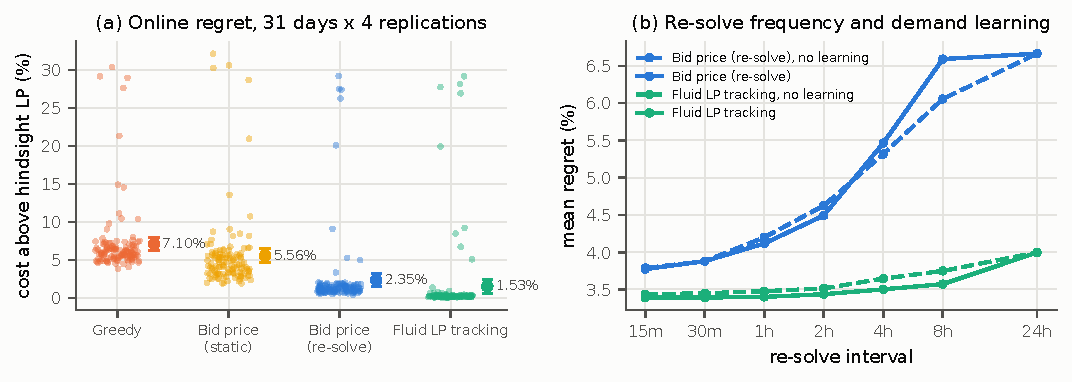
\includegraphics[width=\linewidth]{online}
  \caption{(a) Regret per simulated day; the outliers above 15\% are event days whose demand deviates strongly from the forecast. (b) Mean regret as a function of the re-solve interval, with and without online demand learning (every third test day). LP tracking is far less sensitive to stale information than bid prices.}
  \label{fig:online}
\end{figure}

\Cref{tab:online} and \cref{fig:online} show a clear ranking.
\begin{itemize}
  \item \textbf{Greedy assignment costs 7.1\% more than hindsight}, about \EUR{184}k per day. Most of the loss comes from spot capacity (three times the hindsight volume) and late deliveries. Greedy fills the cheap next-day lanes with the first customers of the day; later customers in other regions then need spot trucks or late lanes.
  \item \textbf{Static bid prices close 22\% of this gap.} That is of the same order as the 36\% reported by \citet{acimovic2015} on industry data with a comparable dual-value heuristic. They fail when the day deviates from the forecast: on 18\% of the days they are worse than greedy.
  \item \textbf{Re-solving hourly closes 67\%}, and \textbf{fluid LP tracking closes 79\%} (regret 1.5\%; 0.3\% on regular days). The policies are separated by \EUR{110}k per day between greedy and LP tracking.
  \item \textbf{Robustness.} Panel (b) explains the difference between the two LP-based policies. Bid prices are \emph{marginal} information: they are only valid locally, and degrade quickly as the state drifts from the one they were computed for (from 3.8\% regret at 15-minute re-solves to 6.7\% with a single solve). Tracking the LP \emph{flows} uses the full primal plan and is almost insensitive to the re-solve frequency (3.4\% to 4.0\%). Multiplicative demand learning brings only small gains, because the day-ahead forecast is already conditioned on yesterday's level.
  \item \textbf{Event days} remain the hardest, with 5.7\% regret even for LP tracking: the forecast error is large and arrives early in the day. This is where intraday re-forecasting and promise-date flexibility would pay most.
\end{itemize}
Computationally, all policies run a full day of about 25{,}000 batch decisions in under half a second, LP solves included. The LP is the same warm-started recourse model used by the planner, re-optimised by dual simplex in milliseconds.
